\subsection{CNN Model}
As we Mention before in the Review Section \ref{review} we follow \textbf{Facial Expression Recognition using Convolutional Neural Networks: State of the Art} Paper\cite{state_of_art} model numebr Five .
on \textbf{fer13} dataset this model follow this Paper \textbf{Learning Social Relation Traits from Face Images} this model Architecture is \textbf{CPNCPNCPCFF} \footnote{ the operations C , P ,N ,F denote to covolutional ,Pooling ,Normalization,Fully Connected } fig 3.1

\begin{figure}
	\centering
	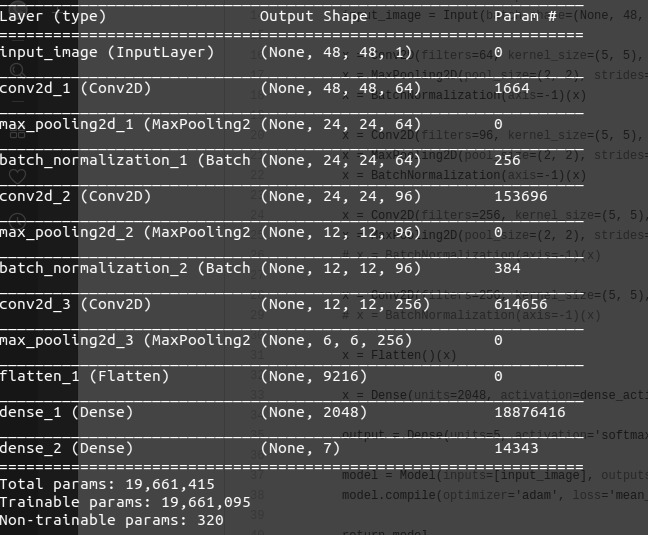
\includegraphics[width=.8\textwidth]{model14.jpg}
	\caption{summary of this model using keras}
\end{figure} 
we get the accuracy mentioned in tabel "3.1"
\begin{table}[h!]
	\begin{center}
		\caption{Tabel of developing Accuracy throw  5 epoches with Batch size 128 and adeleta optimizer \newline}
		\begin{tabular}{l|c|l|c}
			\textbf{Epoch Number} & \textbf{Training Accuracy} & \textbf{Testing Accuracy} &\textbf{Loss}\\ 
			\hline 
			Epoch 1 & 22.08\% & 13.10\% & 3.6658 \\
			Epoch 2 & 22.23\% & 27.96\% & 3.5919 \\
			Epoch 3 & 23.63\% & 18.54\% & 3.7231 \\
			Epoch 4 & 23.10\% & 27.96\% & 3.4896 \\
			Epoch 5 & 24.42\% & 22.89\% &  3.4968 \\									
			\end{tabular}
	\end{center}
\end{table}
\paragraph{Testing accross Multiple Optimizers}
Over a thousand of both training and testing samples and six epoches we get this final values over different optimizers.
\paragraph{After have a quick look to tabel and figure we provide}
we notice that after training this model more and more epoches ,this model fall in Overfitting problem ,we found that no matter how many epoches we run the model at a certin point the testing accuracy be constant and the training accuracy grow and grow without stop.and we notice also the model is unstable having un reasonable change in accuracy . 
\begin{table}[h!]
	\begin{center}
		\caption{Tabel of developing Accuracy with respect to different Optimizers with learning rate 0.01 \newline}
		\begin{tabular}{l|c|l}
			\textbf{Optimizer} & \textbf{Training Accuracy} & \textbf{Testing Accuracy}\\ 
			\hline 
			Adadelta & 38.3\% & 36.3\% \\
			Adagrad & 40.2\% & 33\%\\
			Nadam & 36.8\% & 36\% \\
			Adamax & 37.7\% & 32\% \\
		\end{tabular}
	\end{center}
\end{table}
\paragraph{}
Using the the all dataset with adadelta optimizer ,we get a result of 95\% training accuracy and only 33\% testing accuracy.
\subsubsection{OverFitting and model Stablization}
\paragraph{So we try to Solve this problem }
We found some solutions as :
\begin{enumerate}
	\item Update Layers of Model.
	\item apply Cross Validation Technique.
	\item try Early Stoping Technique.
\end{enumerate}
\subsection{Update Layers of Model}
here we try to update layers of our model making it more simple get the feature we need from each image as fast as we can and try to make the gap between accuracy of training and testing small to be accepted.
\textbf{Keep on your mind that we working on fer13 dataset that is challanging data set so we have a big problem here.}
\subsubsection{New Structure}
Before going through the new structure ,let us discuss
\textbf{what is Batch Normalization?}
\paragraph{Batch Normalization}
As we Know we normalize the input layer by adjusting and scaling the Features. For example, when we have features from 0 to 1 and some from 1 to 1000, we should normalize them to speed up learning. If the input layer is benefiting from it, why not do the same thing also for the values in the hidden layers, that are changing all the time, and get 10 times or more improvement in the training speed.
\paragraph{}
Batch normalization reduces the amount by what the hidden unit values shift around (covariance shift).To explain covariance shift, let’s have a deep network on cat detection. We train our data on only black cats’ images. So, if we now try to apply this network to data with colored cats, it is obvious; we’re not going to do well. The training set and the prediction set are both cats’ images but they differ a little bit. In other words, if an algorithm learned some X to Y mapping, and if the distribution of X changes, then we might need to retrain the learning algorithm by trying to align the distribution of X with the distribution of Y.
Also, batch normalization allows each layer of a network to learn by itself a little bit more independently of other layers.
We can use higher learning rates because batch normalization makes sure that there’s no activation that’s gone really high or really low. And by that, things that previously couldn’t get to train, it will start to train.

\paragraph{}
\textbf{It reduces overfitting}
because it has a slight regularization effects. Similar to dropout, it adds some noise to each hidden layer’s activations. Therefore, if we use batch normalization, we will use less dropout, which is a good thing because we are not going to lose a lot of information. However, we should not depend only on batch normalization for regularization; we should better use it together with dropout.
\paragraph{Back to the new Structure}
We update our structure to be as in this Figure 3.2
\begin{figure}
	\centering
	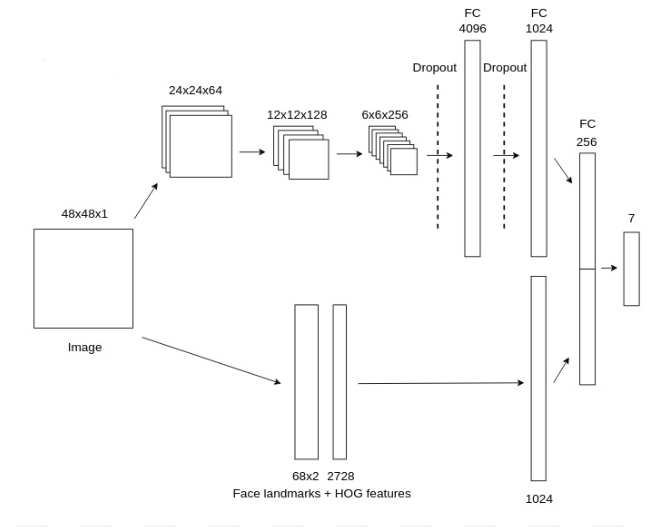
\includegraphics[width=.5\textwidth]{Arch.png}
	\caption{model new Architecture}
\end{figure} 
\paragraph{}
We add Hog and Landmark path as a feature extractor methods 
result of this section without Normalization
!!!!!!!!!!!!!!!!!!!!!!!!!
\paragraph{}
After adding Normalization Layers we get \textbf{testing accuracy of 56.93\%} and\textbf{training accuracy of 74\%} after 10 epochs. 
\paragraph{}
We notice an increase now of the accuracy and more stablization after adding the Normalization layer .
\subsubsection{Apply Cross-Validation}
\subsubsection{Apply EarlyStoping}
 
\subsection{Transfer-learning}
\paragraph{VGG16}
\subsection{Auto-Keras}
\paragraph{}
hee
